\section*{Question 6}

\paragraph{(a)} The two solved models give us the full optimal policy functions for every state $(b, k_t)$ at every age $t$: the baseline $h^*_{\text{base}}(t,b,k)$ and the reform $h^*_{\text{ref}}(t,b,k)$. To simulate the unanticipated reform we splice these at year 8: for years before year 8, each worker follows $h^*_{\text{base}}$ (they do not know the reform is coming, so their optimisation is unchanged); from year 8 onward they follow $h^*_{\text{ref}}$ (they have just learned about $\pi_1$ and respond optimally given their current human capital). The critical difference from the anticipated version is that human capital at year 8 was accumulated under baseline incentives---workers did not build up extra $k$ in anticipation of the subsidy.

\paragraph{(b)}

\begin{figure}[H]
  \centering
  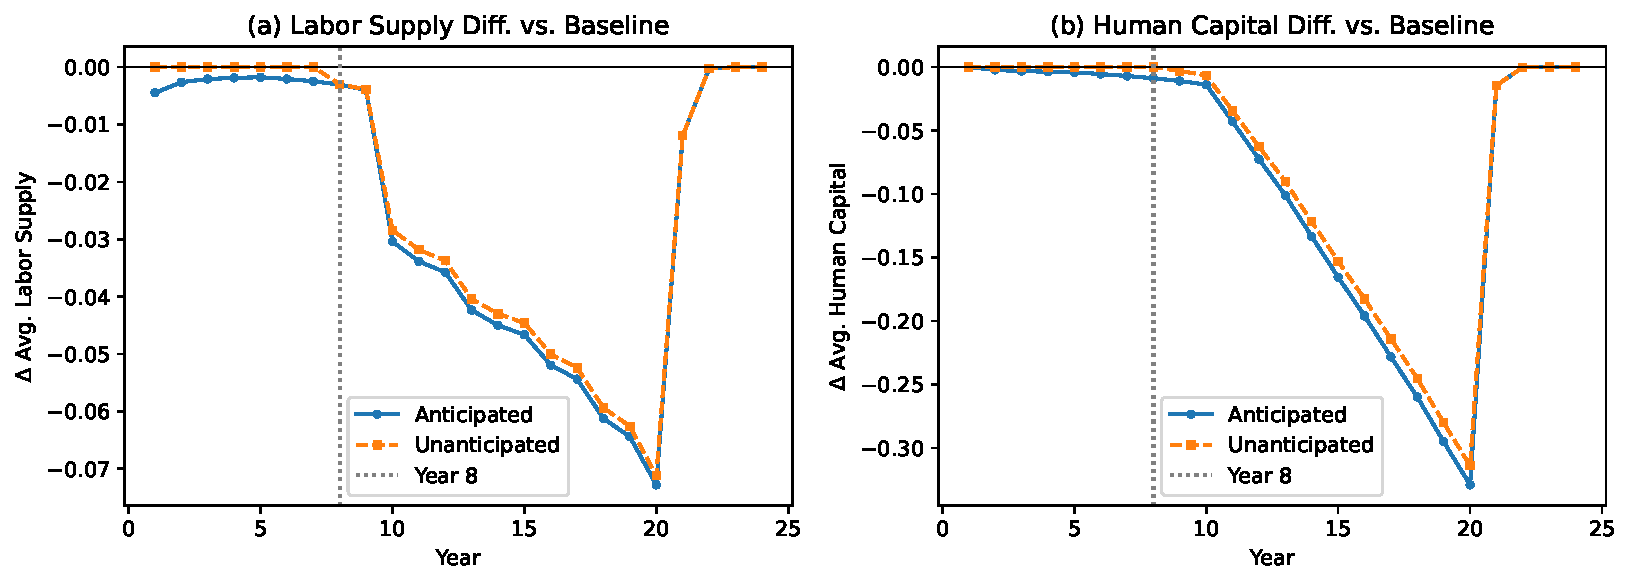
\includegraphics[width=\textwidth]{../figures/q6_comparison_by_year.pdf}
  \caption{Differences relative to the baseline model by calendar year ($\tau_1 = 0$ in all models). \textit{(a)} Labor supply: the anticipated reform shows a small negative anticipation effect from year 1; the unanticipated reform is exactly zero before year 8. From year 8 onward both reforms reduce labor supply, but the anticipated group reduces it slightly more. \textit{(b)} Human capital: anticipated workers accumulate less $k$ from year 2 onward due to reduced hours; unanticipated workers track the baseline exactly until year 8, then diverge.}
  \label{fig:q6}
\end{figure}

\paragraph{(c)} Three patterns stand out. First, the anticipated reform generates a pre-reform behavioral response: workers cut hours slightly in years 1--7, knowing the retirement subsidy is coming. This ``anticipation effect'' is small in magnitude ($\Delta h \approx -0.002$ to $-0.005$) but it compounds into a meaningful human capital deficit by year 8. The unanticipated reform produces no such effect---behavior before year 8 is identical to the baseline by construction.

Second, after year 8 the anticipated group reduces labor supply more than the unanticipated group. The reason is that anticipated workers carry less human capital into the post-reform period (from the pre-reform reduction in hours), so their wages are slightly lower and retirement is marginally more attractive.

Third, the human capital gap between the two reforms widens over time. Because anticipated workers started reducing hours earlier, their $k$ deficit grows each period through the accumulation equation. Unanticipated workers maintain a smaller deficit because they enter year 8 with full baseline human capital.
